%%
%% GMU LaTeX MS Thesis Format Template
%%
%% Developed by:
%%      Daniel O. Awduche and Christopher A. St. Jean
%%      Communications and Networking Lab
%%      Dept. of Electrical and Computer Engineering
%%
%% Notes on usage can be found in the accompanying USAGE_NOTES.txt file.
%%
%%**********************************************************************
%% Legal Notice:
%% This code is offered as-is without any warranty either
%% expressed or implied; without even the implied warranty of
%% MERCHANTABILITY or FITNESS FOR A PARTICULAR PURPOSE!
%% User assumes all risk.
%% In no event shall any contributor to this code be liable for any damages
%% or losses, including, but not limited to, incidental, consequential, or
%% any other damages, resulting from the use or misuse of any information
%% contained here.
%%**********************************************************************
%%
%% $Id: GMU_thesis_template.tex,v 1.16 2007/05/02 02:20:11 Owner Exp $
%%

\documentclass[11 pt]{report}

%%  The file ``gmuthesis.sty''  is the GMU latex style file and
%%   should be placed in the same directory as your LaTeX files
\usepackage{gmuthesis}

%%
%% other packages that need to be loaded
%%
\usepackage{graphicx}                    %   for imported graphics
\usepackage{amsmath}                     %%
\usepackage{amsfonts}                    %%  for AMS mathematics
\usepackage{amssymb}                     %%
\usepackage{amsthm}                      %%
\usepackage[normalem]{ulem}              %   a nice standard underline package
\usepackage[noadjust,verbose,sort]{cite} %   arranges reference citations neatly
\usepackage{setspace}                    %   for line spacing commands

%% The file ``mythesisabbrev.sty'' is an (optional) personalized file that
%% may contain any and all LaTeX command (re)definitions that will be used
%% throughout the document
%\usepackage{mythesisabbrev}

\beforedoc

\begin{document}

%% In this section, all of the user-specific fields to be used in the
%% title pages are set
\title{First line of the title\\
            second line of the title}
\onelinetitle{The complete title is to be repeated here without any line
        breaks for the second page and for the abstract page}
\author{Author}
\degree{Master of Science}
\subject{(Name of Subject)}
\doctype{Thesis}
\dept{(Name of Department)}

\firstdeg{Bachelor of Science}
\firstdegschool{My Former School}
\firstdegyear{Year of first degree}

\degreeyear{Year}

% Note: semester name should be written in its full-form. For example, Fall Semester, not just Fall.
\degreesemester{Semester}

\advisor{Advisor}

\firstmember{First Member}

\secondmember{Second Member}

\depthead{Department Head}

% The current associate dean is Daniel A. Menasc\'{e}
\deanresearch{Dean's Name}

%%
%% Introductory pages
%%

% Note: The signature sheet is set according to the requirements of the Volgenau School of
% Information Technology and Engineering. If your college/school requirement is different,
% please make appropriate changes in the "signaturepage" section of gmudissertation.sty file.
\signaturepage

\titlepage

% copyright technically optional but should be included in to avoid potential pagination problems
\copyrightpage

%%
%% Dedication page
%%

\dedicationpage

\noindent I dedicate this thesis to ...

%%
%% Acknowledgements
%%

\acknowledgementspage

\noindent
I would like to thank the following people who made this possible ...

%%
%% Table of contents, list of tables, and lists of figures
%%

\tableofcontents

\listoftables

\listoffigures

%%
%% Abstract
%%
\abstractpage

The first page of the abstract

%% Be sure to leave a line of whitespace immediately before this line!!!!!
%% (If this comment segment runs together with the preceeding text, you might
%%  see the second page of the abstract numbered "0".)
%%
%% If the abstract is more than one page, then place this line PRECISELY
%% at the page break; otherwise, comment it out.  (See note about this line
%% in the usage notes.)
%%
\abstractmultiplepage

The second page of the abstract

%%
%%  the main body of the dissertation
%%
\startofchapters

%% include the chapters one by one (or paste the chapter text in directly if desired)

%% This file represents a sample first chapter of the main body of the thesis
%%
%%**********************************************************************
%% Legal Notice:
%% This code is offered as-is without any warranty either
%% expressed or implied; without even the implied warranty of
%% MERCHANTABILITY or FITNESS FOR A PARTICULAR PURPOSE!
%% User assumes all risk.
%% In no event shall any contributor to this code be liable for any damages
%% or losses, including, but not limited to, incidental, consequential, or
%% any other damages, resulting from the use or misuse of any information
%% contained here.
%%**********************************************************************
%%
%% $Id: chapterOne.tex,v 1.10 2006/08/25 00:59:32 Owner Exp $
%%

% A first, optional argument in [ ] is the title as displayed in the table of contents
% The second argument is the title as displayed here.  Use \\ as appropriate in
%   this title to get desired line breaks
\chapter[Introduction]{Introduction}

\section{A Section}

A DECLARATION OF RIGHTS made by the Representatives of the good people of VIRGINIA, assembled in full and free
Convention; which rights do pertain to them and their posterity, as the basis and foundation of Government.

\begin{enumerate}
  \item That all men are by nature equally free and independent, and have certain
    inherent rights, of which, when they enter into a state of society, they cannot, by any compact, deprive
    or divest their posterity; namely, the enjoyment of life and liberty, with the means of acquiring and
    possessing property, and pursuing and obtaining happiness and safety.

  \item That all power is vested in, and consequently derived from, the people; that magistrates are their trustees
    and servants, and at all times amenable to them.

  \item That government is, or ought to be, instituted for the common benefit, protection, and security of the people,
    nation or community; of all the various modes and forms of government that is best, which is capable of
    producing the greatest degree of happiness and safety and is most effectually secured against the danger
    of maladministration; and that, whenever any government shall be found inadequate or contrary to these
    purposes, a majority of the community hath an indubitable, unalienable, and indefeasible right to reform,
    alter or abolish it, in such manner as shall be judged most conducive to the public weal.

  \item That no man, or set of men, are entitled to exclusive or separate emoluments or privileges from the community,
    but in consideration of public services; which, not being descendible, neither ought the offices of magistrate,
    legislator, or judge be hereditary.

  \item That the legislative and executive powers of the state should be separate and distinct from the judicative;
    and, that the members of the two first may be restrained from oppression by feeling and participating the
    burthens of the people, they should, at fixed periods, be reduced to a private station, return into that body
    from which they were originally taken, and the vacancies be supplied by frequent, certain, and regular elections
    in which all, or any part of the former members, to be again eligible, or ineligible, as the laws shall direct.
\end{enumerate}


\begin{figure}
  \centering
  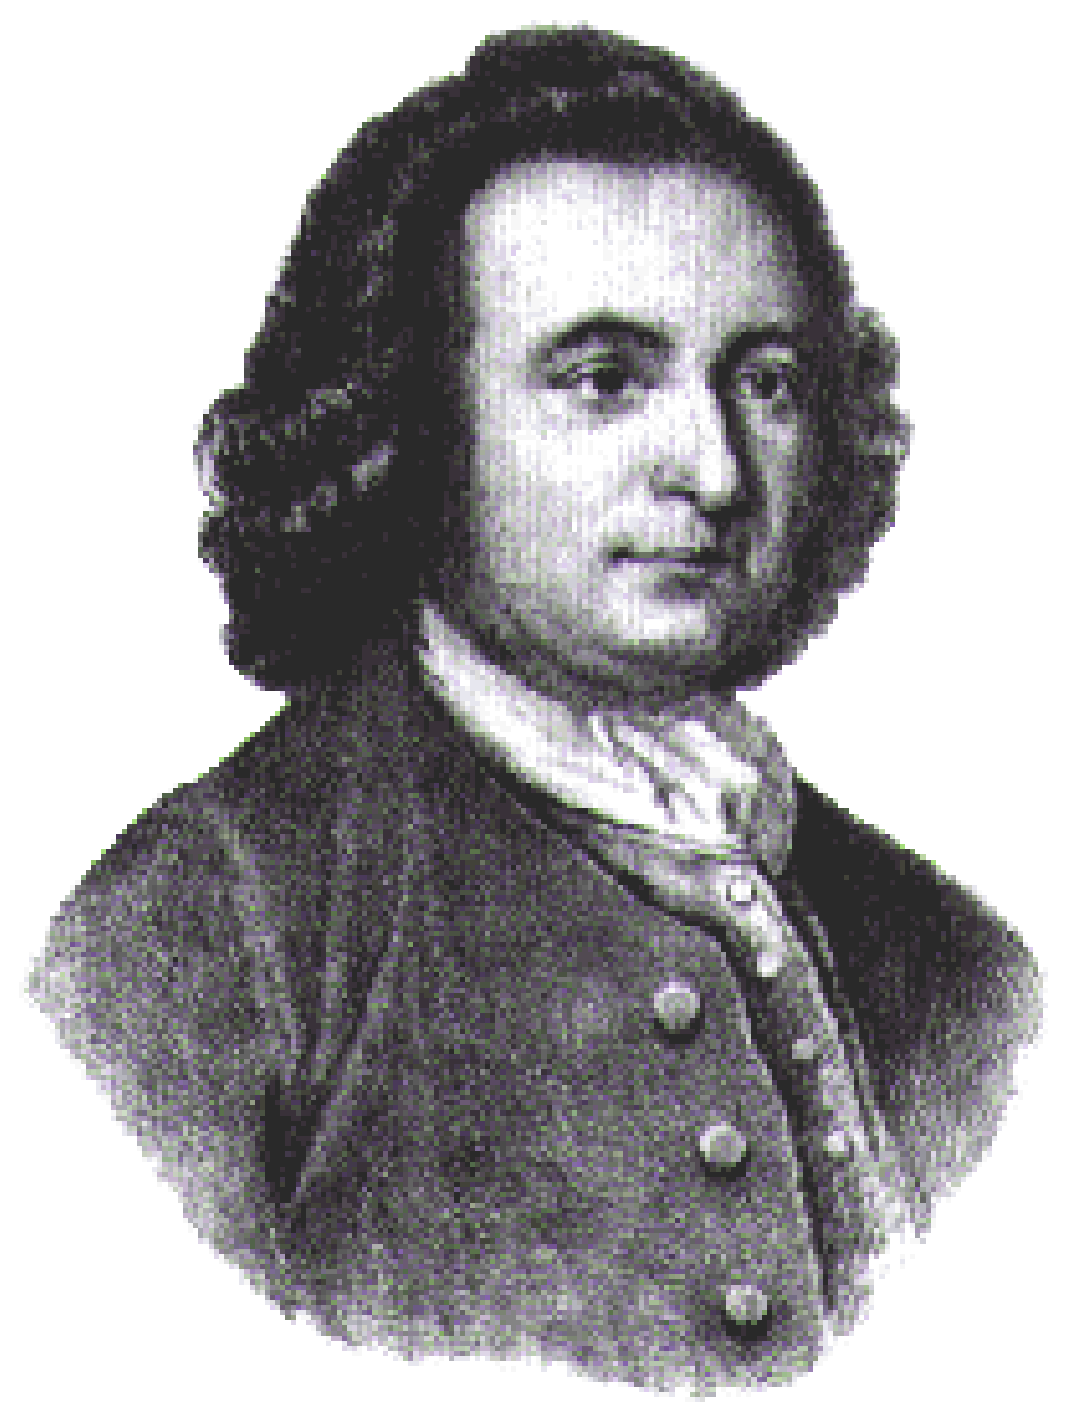
\includegraphics[scale=0.3]{figGeorgeMason}
  \caption[An appropriate historical figure]{An appropriate historical figure.}

  % This adds separation space between this figure and either another figure, or between
  %     the figure and the text.
  \figSpace
\end{figure}

\subsection{A Subsection}

Important previous work was also provided by \cite{Shannon49}.  Here is a numbered equation:
\begin{equation}
    f_X(x) = \lambda e^{-\lambda x} u(x).
\end{equation}

\subsubsection{A subsubsection}

\paragraph{A paragraph}

\subparagraph{A subparagraph}

\begin{table}
  \centering
  \caption{A table}
  % Tabular environment goes AFTER the caption!
  \begin{tabular}{|c|c|c|}
    % after \\: \hline or \cline{col1-col2} \cline{col3-col4} ...
    \hline
    A & B & C \\\hline
    D & E & F \\\hline
    G & H & I \\
    \hline
  \end{tabular}

  % This adds separation space between this table and either another table, or between
  %     the table and the text.
  \tableSpace
\end{table}


\begin{table}
  \centering
  \caption{Another table}
  % Tabular environment goes AFTER the caption!
  \begin{tabular}{|c|c|c|}
    % after \\: \hline or \cline{col1-col2} \cline{col3-col4} ...
    \hline
    1 & 2 & 3 \\\hline
    4 & 5 & 6 \\\hline
    7 & 8 & 9 \\
    \hline
  \end{tabular}

  % This adds separation space between this table and either another table, or between
  %     the table and the text.
  \tableSpace
\end{table}


%% This file represents a sample second chapter of the main body of the thesis
%%
%%**********************************************************************
%% Legal Notice:
%% This code is offered as-is without any warranty either
%% expressed or implied; without even the implied warranty of
%% MERCHANTABILITY or FITNESS FOR A PARTICULAR PURPOSE!
%% User assumes all risk.
%% In no event shall any contributor to this code be liable for any damages
%% or losses, including, but not limited to, incidental, consequential, or
%% any other damages, resulting from the use or misuse of any information
%% contained here.
%%**********************************************************************
%%
%% $Id: chapterTwo.tex,v 1.5 2006/08/25 00:59:50 Owner Exp $
%%


% A first, optional argument in [ ] is the title as displayed in the table of contents
% The second argument is the title as displayed here.  Use \\ as appropriate in
%   this title to get desired line breaks
\chapter[The Second Chapter]{The Second Chapter}

The second chapter begins here.\footnote{This is an example
footnote. We have to add some more words to make sure that we have
more than one line of footnote text to test line spacing.}


%%
%%  bibliography
%%

%% list all of the BibTeX files here for the WinEdt project (if applicable)
%GATHER{bibfile.bib}

%% any bibliography style can be used, but IEEEtran.bst is ideally suited to
%% electrical engineering references

%% include the following directives if there are any appendices
\appendix
\appendixeqnumbering

%% A sample appendix
%%
%%**********************************************************************
%% Legal Notice:
%% This code is offered as-is without any warranty either
%% expressed or implied; without even the implied warranty of
%% MERCHANTABILITY or FITNESS FOR A PARTICULAR PURPOSE!
%% User assumes all risk.
%% In no event shall any contributor to this code be liable for any damages
%% or losses, including, but not limited to, incidental, consequential, or
%% any other damages, resulting from the use or misuse of any information
%% contained here.
%%**********************************************************************
%%
%% $Id: Appendix.tex,v 1.6 2006/08/25 00:58:50 Owner Exp $
%%

% N.B.: an appendix chapter starts with "appchapter" instead of "chapter"
%
% The first argument in [ ] is the title as displayed in the table of contents
% The second argument is the title as displayed here.  Use \\ as appropriate in
%   this title to get desired line breaks
\appchapter[An Appendix]{An Appendix}

This is an appendix.  Here is a numbered appendix equation:
\begin{equation}
    a^2 + b^2 = c^2.
\end{equation}


\bibliographystyle{IEEEtran}
\bibliography{IEEEfull,bibfile}

%%
%% curriculum vitae
%%
\cvpage

\noindent Include your \emph{curriculum vitae} here detailing your background,
education, and professional experience.
\end{document}
